\documentclass{article}
\usepackage[utf8]{inputenc}
\usepackage{amsmath} % Advanced math typesetting
\usepackage[utf8]{inputenc} % Unicode support (Umlauts etc.)
\usepackage[ngerman]{babel} % Change hyphenation rules
\usepackage{hyperref} % Add a link to your document
\usepackage{graphicx}[final] % Add pictures to your document
\usepackage{listings} % Source code formatting and highlighting
\usepackage{bookmark}
\usepackage{natbib}
\usepackage{geometry}
\usepackage{multicol}
\usepackage{fancyhdr}
\usepackage[document]{ragged2e}
 
\pagestyle{fancy}
\fancyhf{}
\fancyhead[LE,RO]{Overleaf}
\fancyhead[RE,LO]{Guides and tutorials}
\fancyfoot[CE,CO]{\leftmark}
\fancyfoot[LE,RO]{\thepage}
\graphicspath{{Immagini/}}

\geometry{
 a4paper,
 total={170mm,257mm},
 left=20mm,
 top=20mm,
 }

\title{Imm algorithm implementation for tracking}
\author{
Paiola Lorenzo 000000 

Zanolli Erik 198852}
\date{January 2020}





\begin{document}

\maketitle



\section*{Introduction}
\justify
The porpouse of this document is the analysis and performance evaluation of an IMM algorithm's implementation in
a sensor grid tracking an object. The object can move with two different model, random walk and unicycle, governed by
 a Markov chain. The goal is evaluate the best trade-off between error on estimated position and real position and number of 
 messagesses involved in tracking

\begin{multicols}{2}
    \section*{Backgound}
    \justify
        Tracking a object with a changing dynamic require propers algorithms and filters. Retriving physical data with
        observations it's not enough, models achiving the best-fit to our data is needed in order to make a prediction and estimate 
        with reduced uncertainty. Here comes to play a major role the IMM algorithm (Interacting Multiple Models): The data
        from sensor are combined with different dynamical models through the algorithm... 
        \subsection*{Simulation Model}
            The target can move with random movement described by a Markov chain and accordingly two different models of movement
            The tracking are performed with grid of sensors. In order to perform a proper simulation the sensor has assumed to have a limited
            range for the tracking and we cannot retrive any information if target is out. It also took in consideration the power consumption 
            for a possible physical system: to model a more enegy efficient system the sensor can switch to 3 different working condition: On,Off,Idle.
            To achive this goal the sensor is working as a state machine as showned in the figure below:
            
            Sensors can communicate with the sensors in their neighboorhoods and exchange signal named CanSense and CantSense that regulate the transition
            between differents state. 

            {How the sensors works}

            The measurment acquired by eachs sensors are then combined through the theory of linear consensus
            The filter choosed are the WSL
            
            Sensors in the simulations are Radar and the H matrix that reprent the measurment:

        \subsection*{m}
    
    \section*{Simulation model implementation}
    Introduction
    \subsection*{Filter}
    \subsection*{Sensor}
    The sensor grid are is composed by a set of sensor that can communicate with each others creating a fully connected graphic
    The single sensor works as a state machine, and change its state accordingly with the signal exchanged with the neighboors.
    \begin{figure}[htp]
        \centering
        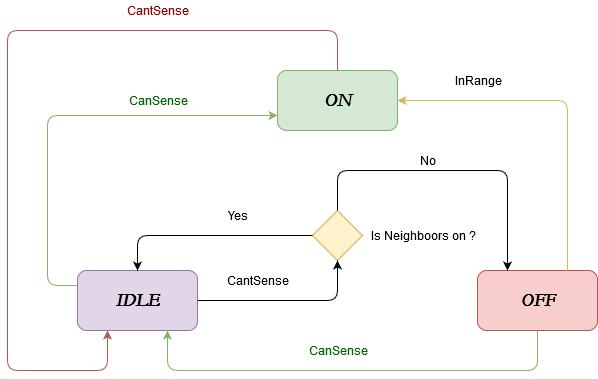
\includegraphics[width=2cm, height=2cm]{UntitledDiagram.png}
        \caption{An image of a galaxy}
        \label{fig:galaxy}
    \end{figure}
    \subsection*{Random walk and Unycicle model}
    The target in this simulation can move accordingly to two model: random walk and Unycicle. The genaral expression of the two process it
    \begin{equation}
    X^{+}=\begin{bmatrix} A \\ \end{bmatrix}X(k)+\begin{bmatrix} B \\ \end{bmatrix}u(k) + \begin{bmatrix} G \\ \end{bmatrix}w(k)
    \end{equation}
    State,state and noise matrix associate to the random walk has showned below:
    $$
    X=\begin{bmatrix} x \\ y \\ \dot{x} \\ \dot{y} \\ \end{bmatrix}
    $$

    $$
    A=\begin{bmatrix}
    1&0&\delta&0\\
    0&1&0&\delta\\
    0&0&1&0\\
    0&0&0&1\\
    \end{bmatrix}
    $$

    $$
    G=\begin{bmatrix}
    \delta^2/2&0\\
    0&delta^2/2\\
    \delta&0\\
    0&\delta\\
    \end{bmatrix}
    $$

    $$
    B= \begin{bmatrix}
        \delta^2/2&0\\
        0&delta^2/2\\
        \delta&0\\
        0&\delta\\
    \end{bmatrix}
    $$
   The unycicle model state representation employed has showned below

    
    \section*{Result}
    The performance evaluation of the system are evaluted by computing the RMS of the predicted trajectory eith the respect to the actual one 
    choosing different rate of performind the WSL. The final result are listed in the table below
    

\begin{center}
    \begin{tabular}{||c c c c||} 
    \hline
    1 step & 2 step & 3 step & 4 step \\ [0.5ex] 
    \hline\hline
    1 & 6 & 87837 & 787 \\ 
    \hline
    2 & 7 & 78 & 5415 \\
    \hline
    3 & 545 & 778 & 7507 \\
    \hline
    4 & 545 & 18744 & 7560 \\
    \hline
    5 & 88 & 788 & 6344 \\ [1ex] 
    \hline
   \end{tabular}
   \end{center}
   
   
    \subsection*{}
\end{multicols}
\end{document}
